\documentclass[lettersize,journal]{IEEEtran}
\usepackage{amsmath,amsfonts}
\usepackage{algorithmic}
\usepackage{array}
\usepackage[caption=false,font=normalsize,labelfont=sf,textfont=sf]{subfig}
\usepackage{textcomp}
\usepackage{stfloats}
\usepackage{url}
\usepackage{verbatim}
\usepackage{graphicx}
\hyphenation{op-tical net-works semi-conduc-tor IEEE-Xplore}
\def\BibTeX{{\rm B\kern-.05em{\sc i\kern-.025em b}\kern-.08em
    T\kern-.1667em\lower.7ex\hbox{E}\kern-.125emX}}
\usepackage{balance}
\begin{document}
\title{Robotic Reconstruction of Islamic Calligraphy Using Twisting Bezier Splines}
\author{Muhammad Umar Hassan, Muhammad Sabieh Anwar and Ali Raza
%\thanks{Manuscript created October, 2020; This work was developed by the IEEE Publication Technology Department. This work is distributed under the \LaTeX \ Project Public License (LPPL) ( http://www.latex-project.org/ ) version 1.3. A copy of the LPPL, version 1.3, is included in the base \LaTeX \ documentation of all distributions of \LaTeX \ released 2003/12/01 or later. The opinions expressed here are entirely that of the author. No warranty is expressed or implied. User assumes all risk.}
}

\markboth{Journal of \LaTeX\ Class Files,~Vol.~18, No.~9, September~2020}%
{How to Use the IEEEtran \LaTeX \ Templates}

\maketitle

\author{Muhammad Umar Hassan, Muhammad Sabieh Anwar and Ali Raza}
%\includepdf{UETFormattedTitlePage.pdf}
\begin{abstract}
\label{Chapter:Abstract}
{
    Automated reconstruction of Islamic architectural calligraphy can save thousands of nobel and historic scripts all over the world from going extinct. One of the fundamental problems in such reconstruction tasks is the absence of a tool that can bridge the gap between artists and the machines (such as a robotic arms) by taking input as conventional calligraphy format and transform into a robot-program. Not just the reconstruction, even in this digital age, no such method exists that lets the artists generate new broad-edge scripts that can be reproduced mechanically. In this context, the research presented herein introduces a novel innovation in the conventional Bezier spline curves to use them to effectively answer the artistic requirements of copying or creating broad-edge calligraphy scripts and can directly produce data needed by the industrial robots. To demonstrate the effectiveness of our approach, two famous scripts are reproduced using the new splines and a comparison is made with the originals. Additionally, to establish how these splines can be used with machines, a robotic simulator is also discussed and the output analyzed both qualitatively and quantitatively. In addition to mechanized reconstruction Islamic calligraphy, the presented approach can also be used for generating calligraphy for virtual 3D models, e.g. in Metaverse, 3D documentation of non-reachable and ruined buildings and even OCR of islamic calligraphy scripts.
}
\end{abstract}

\begin{IEEEkeywords}
Class, IEEEtran, \LaTeX, paper, style, template, typesetting.
\end{IEEEkeywords}
\input{03 - Introduction.tex}
\section{Twisting Bezier Splines}
\label{Chapter:SplineModelling}

    \subsection{The need of twisting bezier splines}
    Conventional bezier curves are commonly used to define outline fonts [cite] and digital calligraphy [cite] due to their ability to accurately trace [cite] the outline of scripts written with and without a broad edge tool [cite]. These curves can be easily manipulated [cite] and rendered [cite] on a computer screen as well as they can be printed on paper. However, in light of the underlaying problem, and in order to preserve the essence of artistic norms [cite], it is desired that a script is written using a conventional broad-edge tool by a robotic manipulator [cite] in a similar fashion to a human artist. Separate techniques [cite] are needed to convert output of the outline or pitch curve functions to a format that a robot can directly use for the desired tool movement. Even though many of these techniques [cite] can promise accurate tracing, none of them can promise that the robot will use the exact tool movement of a human agent.

    In most literal terms, beizer spline curves are sets of decimal values that define the graphical shape of certain mathematical functions [cite]. The input of these functions contains two dimensional points located in the frame of reference of the screen on which they are created and work as handles to control the shape of the curve using a screen pointer. A user can physically relocate these curvature handles on the computer screen and the shape of the resulting spline will follow. The output of these mathematical functions is absolutely repeatable and can be linearly scaled to any units. Usually, a curve is made of up a lot of such lines each with its own set of input coefficients. Although these individual functions are continuous, there output can easily be discretized as closed paths made up of closely located two dimensional points with controllable resolution [cite]. This is exactly the kind of information required by most of computer graphics and printing drivers to render an output.

    Now, as effective as the bezier curves are for screen and paper printing, they still cannot tell how a physical tool should move on a piece of paper to create the desired output. The splines are just organic shaped paths with no thickness. One of the ways to convert them into ink-mark, is to interpret them as the pitch line for a thick round tool tip. This technique is used by plotters [cite] and some hand writing replicators [cite] to produce a written script. However, only a few fonts [cite] can be replicated by this technique. The other technique is to fill the glyph by moving the tool continuously on a path computed by algorithms such as those used by CAD tools [cite] to fill in (or cut) the area contained by the outline of the glyph using a thick round tip tool. The later can produce outputs that looks similar to broad-edge calligraphy but will still not be the same due to the visible tool paths that are not expected when using an actual broad edge tool.

%    Conventionally, image processing is being used [cite] to extract data that can be used to create machine data for calligraphy. We, however, propose a difference; no matter how strong and robust image processing gets, we maintain that there is no alternative to the minor details only a real artist can observe and recreate. So a solution is needed that fulfils the technical needs as well as the artistic demands. One can virtually draw any kind of shape that can be represented on a two dimensional surface using the conventional bezier splines but it is not very intuitive to accurately reproduce the output of a broad-edge tool.

    On the other hand, twisting bezier splines, instead of working as outline curves, directly record the pitch line of a twisting broad-edge tool stroke along-with the twist information and recreate the live result to the artist who can than morph the spline in a convenient way as normal splines. Their usage is just as intuitive as the conventional bezier splines and will be demonstrated in the next sections, and the information they contain can not only be used to render the script back on the screen or a photo printer, but also be directly considered as machine data for robotic manipulators.

    In contrast to normal bezier splines, twisting bezier splines not only trace the pitch lines of all the strokes but also the twist of the tool independent of the curvature. This is done by introducing another input to the curve function that we call the ``rotation'' or ``twist'' handle. Just like the curvature handles represent the function inputs responsible to define the curvature of the pitch line which is in fact a normal spline, the rotation handles represent the inputs that control the twist of the simulated broad-edge tool. Just like conventional bezier splines, functions of the twisting bezier splines can also be discretized and converted into a list of two dimensional list of points; a closed path to emulate the ink-mark of the broad edge tool. As was the case with normal splines, this is exactly the kind of data needed by the computer display drivers.

    Interestingly, although the twisting splines originate on a computer screen, they are still nearer to the machine than they are to computer graphics data. To compute the list of the points needed to create a filled path that represents the ink-mark, a broad edge tool is emulated to be moving on the rotating spline with the twist also controlled by the spline. In actuality, the emulated tool is replaced by a real tool that can be mounted on a robotic manipulator. The spline directly controls the position and twist of the tip of a tool which can directly be translated into machine movement codes. The rest of the process for painting involves inverse kinematics [cite] and is already handled by the robot controller.

    \subsection{Mathematical Model of a Twisting Bezier Spline}
    \subsubsection{The Conventional Bezier Spline}
         We first describe conventional bezier splines. Figure \ref{Fig:BezierSplines} illustrates different aspects of a spline path composed of several sub curves. Each curve section is only partly independent of the other. Figure \ref{Fig:BezierSplines} (a) shows how individual splines combine to form a bigger spline path. These sections are labeled $1$ through $5$. Figure \ref{Fig:BezierSplines} (b) shows anchors and curvature handles of each part of the path. For instance, Figure \ref{Fig:BezierSplines} (c) extracts and highlights section $4$ and shows anchor points $A$ and $B$ that control this section. Each anchor has two handles referenced from its position. For example, anchor $A$ has two handles, $H_1$ and $H_2$, connected through a straight line passing through the parent anchor and referenced from the parent anchor. Overall, handles $H_1$, $H_2$, $H_3$ and $H_4$ are attached to the two anchors that control this section, however in addition to the anchors, only $H_2$, $H_3$ are directly responsible to control the curvature of this section. It must be noted here that although the lengths of segments $\overline{AH_2}$ and $\overline{BH_3}$ are not connected to the lengths of segments $\overline{AH_1}$ and $\overline{BH_4}$ respectively, the positions of handles $H_2$ and $H_3$ are also influenced by $H1$ and $H4$. These handles control the curvature of the neighboring sections $3$ and $5$ and thus indirectly influence the shape of section $4$ as well. This is how each section is only partly independent and connected to neighbouring sections.



        \begin{figure}[!t]
            \centering
            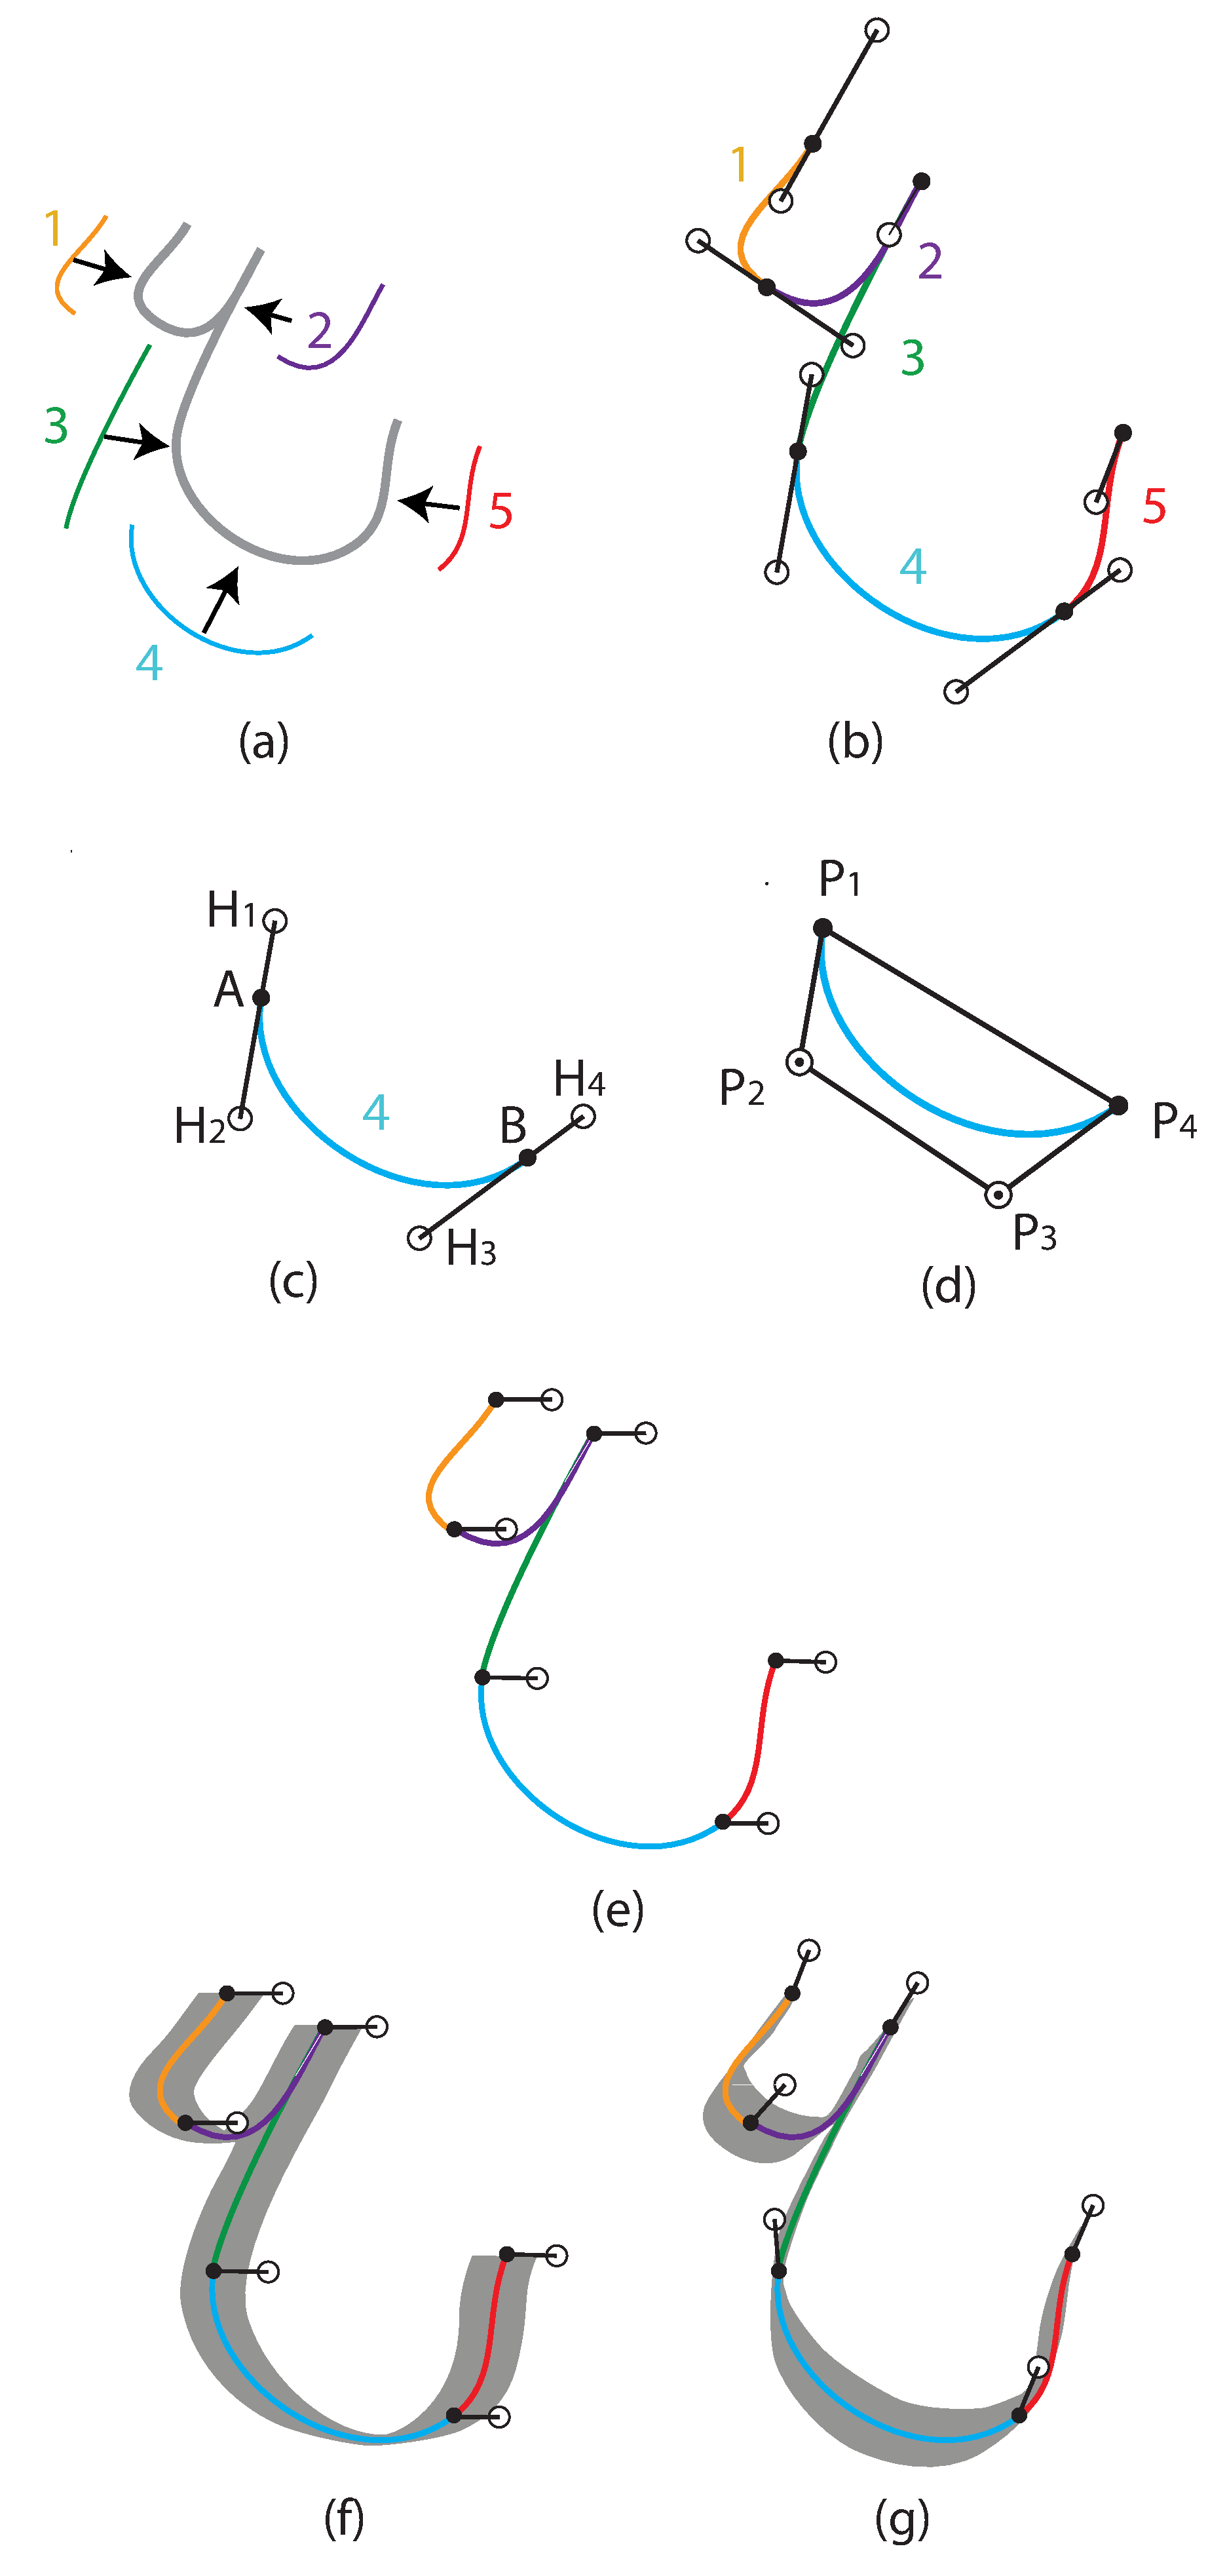
\includegraphics[width=2.5in]{../Images/BezierSplineCurve.pdf}
            \caption{The figure first illustrates how a spline is constructed and is transformed to a twisting bezier spline. (a) An exploded view of a bezier spline path that show the individual splines that compose the parent path. (b) Control handles and anchors appear at the junctions of two consecutive splines. (c) One portion of the spline path, its handles and anchors are highlighted. (d) The relevant handles and anchors of the spline are connected to form a construction polygon. (e) Horizontally oriented rotation handles are attached to each anchor of the parent spline path. (f) A continuous inkmark sweeps the spline path with the tool rotation controlled by horizontally oriented rotation handles. (g) The position of rotation handles is adjusted and fine tuned to get the desired shape of the inkmark. }
            \label{Fig:BezierSplines}
        \end{figure}

        Now, it may look like the shapes defined in this way are pretty organic but in fact, the whole shape is defined by simple mathematical equations. Figure \ref{Fig:BezierSplines} (d) focuses on section $4$ and $5$ of the curve and also shows a polygon defined by the points $P_1$, $P_2$, $P_3$ and  $P_4$. It must be noted that the points $P_1$ and $P_4$ of this polygon are also the anchor points between sections $3$, $4$ and $5$. Take section $4$ for example. The polygon mathematically defines the complete shape of this curved part. If $P_{spline}$ is a point on section $4$, with coordinates $x$ and $y$ in a Cartesian plane referenced to some origin, it is defined as
         \begin{equation}
         \label{splineModel01}
         P_{spline}=P_b×f+P_a×(1 -f).
         \end{equation}
where,
\begin{equation}
\label{splineModel02}
P_a=P_{23}×f+P_{12}×(1 -f)
\end{equation}
and
\begin{equation}
\label{splineModel03}
P_b=P_{34}×f+P_{23}×(1 -f)
\end{equation}
where,
\begin{align}
P_{12}&=P_2×f+P_1×(1 -f), \\
P_{23}&=P_3×f+P_2×(1 -f)
\end{align}
and
\begin{equation}
\label{splineModel04}
P_{34}=P_4×f+P_3×(1 -f)
\end{equation}
and, $f \in [0, 1]$.

It can also be proved that the side segments of the polygon $\overline{P_1 P_2}$ and $\overline{P_3 P_4}$ are tangent to the curve at the point they meet it at $P_1$ and $P_4$ respectively.


\subsubsection{Twist Handle}
    On top of the conventional bezier splines that work around anchor points possessing curvature handles, we add a ``rotation'' or ``twist'' handle to each anchor and one scalar thickness parameter to the whole curve. The thickness parameter defines the length of a flat line segment centered on $P_{spline}$, oriented arbitrarily at a constant angle with reference to the curve origin and, sweeping on the curve to form a two dimensional region representing the inkmark. We then define the orientation of this line segment as it sweeps along as a linear function of three variables. First, is the fractional position of the center of the segment which is the same as $f$. The second and third variables are the two angles that are subtended by the rotation handles about their respective anchors with respect to the horizontal axis. This means that the orientation of the sweeping line when located exactly on a particular anchor is the same as the angle between the twist handle and the center of the respective anchor. Figure \ref{Fig:BezierSplines} (e) shows rotation handles added in the example under discussion. It must be noted that the curvature of the spline remains the same even after adding twist handles that are lying horizontally yet. The swept inkmark region is shown in Figure \ref{Fig:BezierSplines} (f). Figure \ref{Fig:BezierSplines} (g) shows the final form of the twisting bezier spline after the twist handles have been iteratively moved to positions that impart the spline with the desired look.

    In simpler words, it is similar to sweeping a broad-edge pen centered on the actual spline while twisting it uniformly and continuously about its own axis at an angle
    \begin{equation}
    \theta_{twist}=\theta_A  (1-f)+ \theta_B
    \end{equation}
    with respect to the horizontal axis. Here $f$ is the same factor that was used to define $P_{spline}$ and $\theta_A$ and $\theta_B$ are the absolute angles subtended by the first and the second anchor and their respective rotation handles measured from the horizontal axis. It may be noted that since each anchor is connecting two adjacent sub curves, the ending angle of the sweeping line at the end of the first curve is always the same at the beginning of the latter. This obscures the visual transition of the twisting curve from one sub curve to the other.

    It must also be noted that the angle of rotation handle cannot be constrained in a $2\pi$ domain. Instead, it is completely unbounded, and the sweeping pen may actually take multiple turns both clockwise and anticlockwise while moving on a single curve section as well as the whole curve.

    \subsection{Digitization of Calligraphy Artwork}
    Using twisting bezier splines we can include the artists in the process of digitization of existing calligraphy work. An open source tool called ``Gregor'' [link to source] is available that can create, modify, save, and reload rotating bezier splines. With this tool, one can also manually trace existing calligraphy work available in the form of computer images. One can also extend the tool to automate the tracing process by creating a curve fitting technique that tries to fit the output image of the rotating bezier splines on the existing ink-marks in the photos by iterating the coefficients of the spline to minimize the count of pixels in the difference of both images.

    \subsection{Machine Data Generation}
    \label{ExplorationPoints1}
    The rotating spline curves are themselves emulated ink-marks of a broad edge marking tool. This is the reason extracting machine data and even G-codes from them becomes natural. The minimum information required by a robot to draw a broad-edge stroke trickles down to the definition of the path on which the pen must move and the twist of the pen in the world coordinates. Except for the information about a three dimensional reference system, this is exactly the information that a typical rotating bezier spline contains. In other words, to call the rotation bezier splines ``machine data'', the following assumptions must be made:

    \begin{itemize}
        \item The flat tip of a broad edge tool is always completely touching the drawing area.
    	\item The inclination of the pen with respect to the drawing area or with respect to the direction of the drawing is either normal or always fixed at an angle which is set by the machine.
    	\item For each tool with different tip width, a separate spline will be used.
    	\item The axial pressure a pen inserts on the drawing board while drawing is also fixed and is set by the machine as well.

    \end{itemize}

    It is worth mentioning that just like the rotation handle gives the axial rotation information, it is intuitive to add more handles to govern more parameters like pen inclination, tool thickness during a stroke, and normal pressure. The effect of varying thickness will appear right on the screen but to visualize the effect of varying pressure or inclination of the pen will have to be displayed using some $3$~D tool visualization, color coding or a similar data presentation technique.

\section{Performance and Bechmarking}
\label{Chapter:Performance}

\subsection{Characterization}
An important aspect of fabricating a new technique is measuring how well it performs in different usage scenarios. Developing a metrics for judging the artistic quality of a calligraphy specimen produced by the Bezier or rotating Bezier splines is altogether a separate discussion and out of scope of this research. However, there are some aspects that we have tried to measure the effectiveness of the rotating splines.

\subsection{Supported Scripts}
All the scripts that are written with rigid broad-edge tools, such as broad-edge pens and markers, where the tool keeps complete contact with the surface throughout the stoke. However, if script requires changing the extent of tool contact with the surface, the best alternate to achieve a similar appearance of the script would be to use multiple splines with multiple thicknesses that overlap each other in a gradual manner. The rotating bezier splines cannot control the tool inclination and applied pressure, therefore, they are not suitable for scripts written with flexible tools like broad-edge brushes.

\subsubsection{Coverage}
To benchmark the performance and accuracy of rotating bezier splines, some test results are presented here. These values are produced by comparing high resolution binary images of actual scripts, extracted with Adobe Photoshop and rasterized images produced by the twisting bezier splines originally formed by tracing the processed images. The pixel density is set such that a pixel-pixel comparison can be performed between the original image and the rasterized splines. The accuracy is analysed by computing the overflow and underflow of the ink by matching pixels of both images. Table \ref{Table:Accuracy} shows a summary of these benchmarks.

\begin{table}
\begin{center}
\caption{Benchmark of the mathematical accuracy of the twisting bezier spline curves}
\label{Table:Accuracy}
\begin{tabular}{| c | c |}
  \hline
\textbf{Metrics} & \textbf{Results} \\
  \hline
Area over flow & $<$ 2\% \\
  \hline
Coverage & $>$ $94\%$ \\
  \hline
Lateral deviation from the pitch line & N.A. \\
  \hline
Compatibility & All broad edge scripts \\
  \hline
Total splines measured & $>100$ \\
  \hline
Total pixels compared & $9.9$~million \\
  \hline
Tested scripts & Nastaleeq, Thuluth \\
\hline
\end{tabular}
\end{center}
\end{table}
%
%This metrics is comprehensive but still not complete. Some additional metrices are still needed to give a verdict about how good the proposed solution is and it is now up to the community to evolve these curves according to the needs. Table \ref{Table:AdvancedMetrices} presents a couple of those metrices that may also be desired by the researchers.
%
%\begin{table}
%\begin{center}
%\caption{Advanced metrices to gauge the effectiveness of twisting bezier splines.}
%\label{Table:AdvancedMetrices}
%\begin{tabular}{| c | c |}
%  \hline
%  \textbf{Metrics} & \textbf{How can it be measured} \\
%  \hline
%Easy of usage & A survey based on Likert scale \\
%  \hline
%Time efficiency of tracing & Comparison of the time taken by the same artists tracing with conventional and rotating Bezier splines \\
%  \hline
%The artistic quality of the specimens produces. & A survey based on Likert scale and filled by a wide range of artists \\
%  \hline
%\end{tabular}
%\end{center}
%\end{table}

% Please note that the third metrics in Table \ref{Table:AdvancedMetrices} seems potent for gauging the performance of atypical supline but is no longer valid given the nature of fabricated splines.

\subsubsection{Sample Results}
As a test and a tribute, two scripts by the famous teacher, artist and author of $18$ calligraphy books, late Khursheed Gohar Qalam \cite{bib23} of the National College of Arts (NCA) were borrowed; one in Nastaleeq and other in Thuluth. Figure \ref{Fig:Nastaleeq} and Figure \ref{Fig:Thuluth} show the bezier spline sets created by tracing both scripts respectively. Figure \ref{Fig:Nastaleeq}(a) and Figure \ref{Fig:Thuluth}(a) show the images of both script samples. Figure \ref{Fig:Nastaleeq}(b) and \ref{Fig:Thuluth}(b) are the rotating splines created by manually tracing the originals. Figure \ref{Fig:Nastaleeq}(c) and \ref{Fig:Thuluth}(c) highlight individual overlapping spline strokes. [Question: Who traced these scripts?]. Table \ref{Table:AdvancedMetrices} shows a quantitative measure of accuracy for these script traces. 

It must also be noted that since the original script image is not available in a sufficiently high digital quality, the digitization and preprocessing error also contributes to the final error in under and over flow of the rotating bezier splines.

    \begin{figure}[!t]
    \centering
    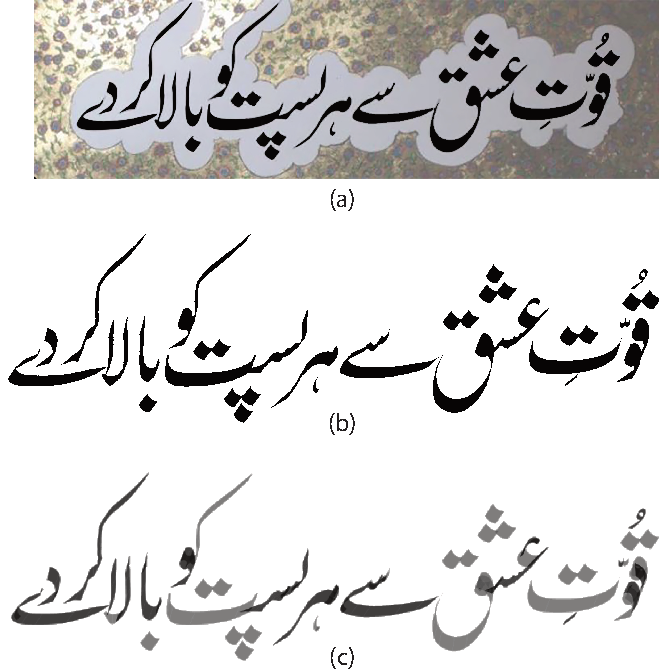
\includegraphics[width=2.5in]{../Images/NastaleeqSample.pdf}
      \caption{
        A specimen produced in ``Nastaleeq'' script. (a) Original photograph of the specimen (b) Rasterized binary image of the twisting spline curves. (c) Rasteriezd shaded image of the twisting spline curves highlighting individual curve parts.}
      \label{Fig:Nastaleeq}
    \end{figure}


    \begin{figure}[!t]
    \centering
    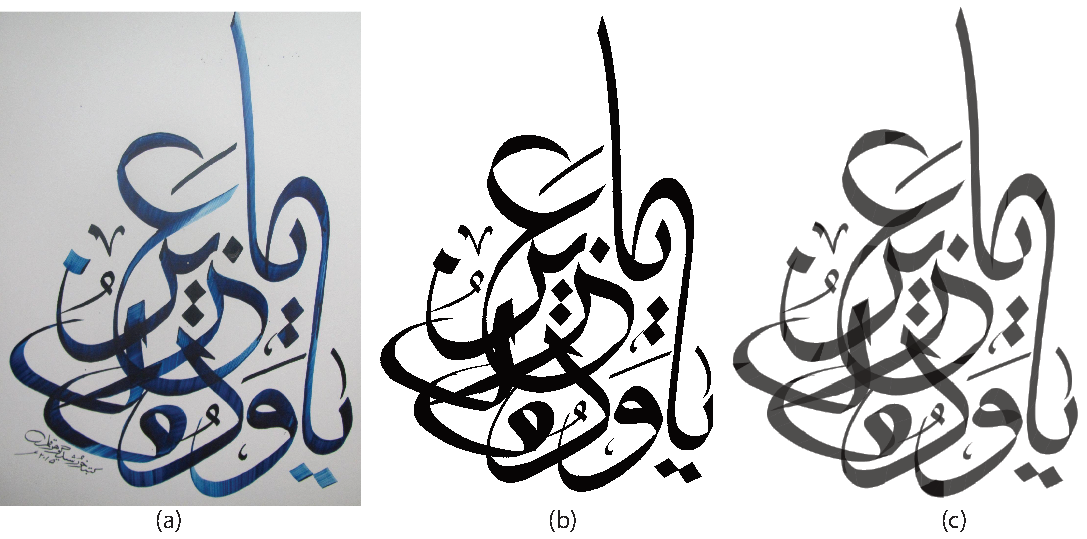
\includegraphics[width=2.5in]{../Images/ThuluthSample.pdf}
    \caption{
        A specimen produced in ``Thuluth'' script. (a) Original photograph of the specimen (b) Rasterized binary image of the twisting spline curves. (c) Rasteriezd shaded image of the twisting spline curves highlighting individual curve parts.
    }
  \label{Fig:Thuluth}
\end{figure}

\subsubsection{Machine Data Generation and Simulation}
    To check how accurately the data generated by these splines can be traced by an actual robotic manipulator, a computer simulation was used. We use an open-source simulator, developed  tailor made for the task. The simulator assumes an open loop [type] robot powered by stepper motors with controllable step size. To generate machine data, the simulator first rasterizes the whole spline with a variable resolution such that the distance between two adjacent points is always smaller than and required linear resolution. To fulfil this requirement for a point $N + 1$ on the discrete spline, the program iterates the fraction $f$ in the spline model [how do we refer to multiple equations?] to minimizes the error between the required resolution and the linear distance between $N$ and $N + 1$. For each computed $f$, the program then calculates the twist component. The set of these the two coordinates of each computed point and the twist component against $f$ defines the position and twist about the normal axis for the tool. The program then transforms this rasterized curve on to an emulated flat writing surface placed in a three dimensional space with some user-set position and orientation. To switch from one spline to the other, the program also adds some additional target points in the array of these points that will lift the tool normally upwards from the writing surface. Finally, the simulator tries to travel on this array of points at a constant speed. 
    
    [Description 1]
    To emulate the writing pen, whenever the simulator detects that the distance of the tip of the tool lies within a configurable thin range, the program records the position and the twist component of the tool on every simulation step. The array of these points is connected using a $3$~D polygon that can be visualised on the screen. The $2$~D projection of this polygon on to the writing pad is extracted to be processed for the pixel-to-pixel comparison with the original script and the ideal rotating spline. The summary of these tests is shown in Table \ref{Table:MachineDataMetrices}.

    [Alternate shorter description]
    For the sake of analysis, in parallel, the end effector orientation is captured continuously to construct an ink mark with each sweep of the tool. The reproduced image is then used for analysis. The results of such a comparison can be seen in Table \ref{Table:MachineDataMetrices}.

    \begin{table}
    \begin{center}
    \caption{Benchmark of the mathematical accuracy of the twisting bezier spline curves with a simulated manipulator}
    \label{Table:MachineDataMetrices}
    \begin{tabular}{| c | c | c | c |}
    \hline
      & \textbf{Reference} & \textbf{Coverage} & \textbf{Extra} \\
      \hline
      \multicolumn{4}{|l|}{\textbf{Nastaleeq}}\\
      \hline
      Rotating Bazier Spline & Original Image & 95.8\% & 5.4\% \\
      \hline
      Machined Output & Original Image & 96.7\% & 7.0\% \\
      \hline
      Machined Output & Rasterized Image & 96.7\% & 4.3\% \\
      \hline
      \multicolumn{4}{|l|}{\textbf{Thuluth}}\\
      \hline
      Rotating Bazier Spline & Original Image & 93.4\% & 2.8\% \\
      \hline
      Machined Output & Original Image & 95.0\% & 3.4\% \\
      \hline
      Machined Output & Rasterized Image & 97.8\% & 4.4\% \\
    \hline
    \end{tabular}
    \end{center}
    \end{table}         % Twisting Bezier Splines
\section{Conclusion}
\label{Chapter:Conclusion}
{
    The accuracy analysis presented in this article demonstrates how rotating bezier splines closely mimic the ink mark of broad edge writing tools thus creating accurate calligraphy scripts. They can be traced on photos of existing calligraphy scripts while also involving the artists to better preserve the artistic spirit. Their resemblance with normal bezier splines makes the learning curve lean for the people who are not accustomed with engineering software and tools. Once traced, they can directly generate machine data for robotic reconstruction and be reproduce the original script on flat and uneven surfaces. Tracing accuracy, ease of use and the ability to generate machine data makes them a strong candidate, not just for Islamic calligraphy but also other broad-edge scripts, to bridge the gap between machines and artists to reproduce and innovate in this field.

    Furthermore, rotating bezier splines can be involved in optical character recognition of Islamic scripts. Since they can be regarded as mathematical curves of the actual ink-marks, a modified curve-fitting technique can be developed to find the perfect curve to match a particular calligraphy script. At the least, the open-source proof-of-the-concept editor presented in this research can be mixed with such a curve fitting tool to help fine tune the manual tracing process.
} 
\begin{thebibliography}{99}
\bibitem{bib01} Web page of Baytulhabeeb, an artist, \url{https://bit.ly/islamic_cal_history}, accessed on Sep 4, 2020.
\bibitem{bib02} Arabetics™, a private foundry and consulting firm, specializing in Arabic type and lettering designs, “Roots of Modern Arabic Script:  From Musnad to Jazm”, \url{https://bit.ly/islamic_cal_history_2}, accessed on Sep 4, 2020.
\bibitem{bib03} “Islamic Calligraphy”, \url{https://bit.ly/Islamic_cal_wiki}, accessed on Sep 4, 2020.
\bibitem{bib04} By Julia Kaestle , “Arabic calligraphy as a typographic exercise”, \url{https://bit.ly/cal_styles}, accessed on Sep 4, 2020.
\bibitem{bib05} Haji Noor Den, Portfolio, \url{http://www.hajinoordeen.com/about.html}, accessed on Sep 4, 2020.
\bibitem{bib06} Mohammad Zakrya, Portfolio, \url{https://mohamedzakariya.com}, accessed on Sep 4, 2020.
\bibitem{bib07} Kamel Al Baba, Mokhtar Al Baba, Portfolio, \url{http://www.arabiccalligraphy.com}, accessed on Sep 4, 2020.
\bibitem{bib08} Abed Yaman, “A look at the history of Arabic calligraphy” \url{https://bit.ly/islamic_cal_stages}, accessed on Sep 4, 2020.
\bibitem{bib09} M. A.-de Lemos, and E. V. Liberado, “Industrial robotics applied to education”, Proceedings of 2011 International Conference on Computer Science and Network Technology.
\bibitem{bib10} Robotics in Agriculture: Types and Applications, \url{https://bit.ly/ind_robots_in_agri}, accessed on Sep 4, 2020.
\bibitem{bib11} A robot playing table tennis, \url{https://www.kuka.com/timo}, accessed on Sep 4, 2020.
\bibitem{bib12} A printing robot, \url{https://bit.ly/ind_robot_cal}, accessed on Sep 4, 2020.
\bibitem{bib20} Project code repository on GitHub, \url{https://github.com/umartechboy/Thesis_2017-MS-MC-17}|, accessed on August 8, 2021.
\bibitem{bib13} M. Bilal, A. Raza, M. Rizwan, M. Ahsan, H. F. Maqbool, S. Abbas Zilqurnain Naqvi, “Towards Rehabilitation of Mughal Era Historical Places using 7 DOF Robotic Manipulator”, in Proceedings, IEEE International Conference on Robotics and Automation in Industry, pp. 1-6, 2019.
\bibitem{bib14} GIMP, GNU Image Manipulation Program Developers Resources, \url{https://bit.ly/gimp_developers}, accessed on July 7, 2021.
\bibitem{bib15} Inkscape Extensions, \url{https://bit.ly/inkscape_developers}, accessed on July 7, 2021.
\bibitem{bib16} Wacom Intuos, \url{https://bit.ly/wacom_intuos_official}, accessed on July 7, 2021.
\bibitem{bib17} Lenovo Thinkpad x380, \url{https://bit.ly/lenovo_thinkpad_x380}, accessed on July 7, 2021.
\bibitem{bib18} Microsoft Surface Pro 7, \url{https://bit.ly/ms_surface_pro_7}|, accessed on July 7, 2021.
\bibitem{bib19} George R. R. Martin, \emph{``A Game of Thrones''}, Chapter $30$.
\bibitem{bib21} \emph{Solving a 6 DoF Robot}, \url{https://bit.ly/SolvingA6DoFRobot}, accessed on November 30, 2021.
\bibitem{bib22} Microsoft .Net Framework, \url{https://bit.ly/ms_dotnet_framework}, accessed on Jan 09, 2022.
\bibitem{bib23} Khursheed Gohar Qalam, \url{https://bit.ly/gohar_qalam}, accessed on Jan 09, 2022.
\bibitem{bib24} Java graphics \url{https://www.javatpoint.com/Graphics-in-applet}
\bibitem{bib25} DotNet graphics \url{https://dotnettutorials.net/lesson/graphics-in-applet/}
\bibitem{bib26} Direct2D Graphics \url{https://docs.microsoft.com/en-us/windows/win32/direct2d/the-direct2d-api}
\bibitem{bib27} G-Codes \url{https://gcodetutor.com/cnc-machine-training/cnc-g-codes.html}
\bibitem{bib28} TTF and OTF Introduction \url{https://docs.microsoft.com/en-gb/typography/opentype/spec/glyf}
\bibitem{bib29} Calligraphy With Photoshop Paperback – December 31, 2004.
\bibitem{bib30} Digital Hand Lettering and Modern Calligraphy: Essential Techniques Plus Step-by-Step Tutorials for Scanning, Editing, and Creating on a Tablet Paperback – Illustrated, August 27, 2019
\bibitem{bib31} Vector Graphics and Illustration: A Master Class in Digital Image-Making Paperback – October 1, 2008.
\bibitem{bib32} S. Wang, J. Chen, X. Deng, S. Hutchinson, and F. Dellaert, ``Robot Calligraphy using Pseudospectral Optimal Control in Conjunction with a Novel Dynamic Brush Model,'' in IEEE/RSJ Intl. Conf. on Intelligent Robots and Systems (IROS), pp. 6696–6703, IEEE, 2020.
\bibitem{bib33} S. Mueller, N. Huebel, M. Waibel, and R. D’Andrea, ``Robotic calligraphy - learning how to write single strokes of Chinese and Japanese characters,'' in IEEE/RSJ Intl. Conf. on Intelligent Robots and Systems (IROS), pp. 1734–1739, IEEE, 2013.
\bibitem{bib34} Josh H. M. Lam and Y. Yam, ``Stroke Trajectory Generation Experiment for a Robotic Chinese Calligrapher Using a Geometric Brush Footprint Model,'' in IEEE/RSJ Intl. Conf. on Intelligent Robots and Systems (IROS), pp. 2315–2320, IEEE, 2019.
\end{thebibliography} 
\end{document}


